%
% The proposed approach is divides in two parts: first, we define a systematic way for a designer specify deployment restrictions to the goal model of the system. Each plan is associated with required computing environment context. We present a Tropos metamodel extension for specify computing environment resources and plans computing environment dependencies.
%
% Second, we introduce an approach for execute the deployment for a given computing environment. The deployment process here encompass deciding with computing resources will be responsible for executing each plan (respecting dependencies restrictions), and which operation needs to be executed in order to realize the deploymet.

%The complete deployment process is illustrated in figure \ref{fig:deployment_process_flow}.

\subsubsection{Roles}
The proposed process considers three roles: users, requirements engineers and software architects.
 Figure~\ref{fig:process_roles} summarize the collaboration between the roles.

\begin{description}
  \item[User]
  This role has access to a particular computing environment and want to achieve some goals there.
  \item[Requirements Engineer]
  Is responsible to translate users goals to a contextual goal model. Also is responsible to analyze the different contexts that the system is meant to operate and how it affects the goals.
  \item[Architect] Architect project the software architecture such as to permit variability of deployment.
  From the point of view of dynamic heterogeneous computing environments, the focus is to create interfaces for components that can allow for goal achievements using different computing resources.

\end{description}

\begin{figure}[!htb]
  \centering
  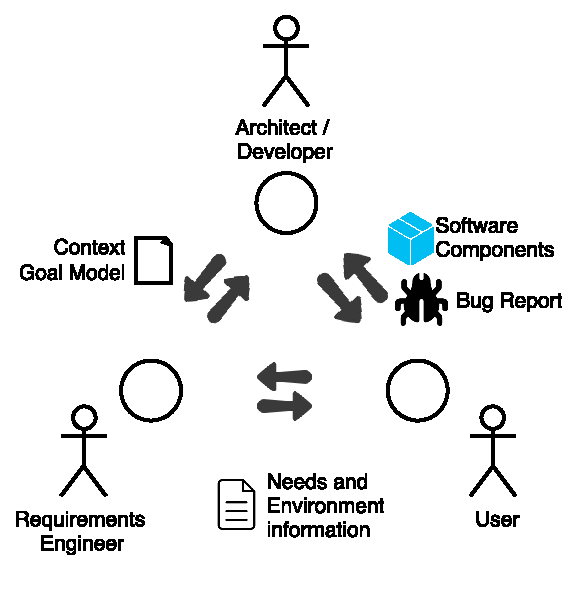
\includegraphics[width=.6\linewidth]{process_roles}
  \caption{Roles collaboration}
\label{fig:process_roles}
\end{figure}

\subsubsection{Activities}

Figure~\ref{fig:deployment_process_flow} describe the development process activities.

\label{sub:Proposal}
\begin{figure}[!htb]
  \centering
  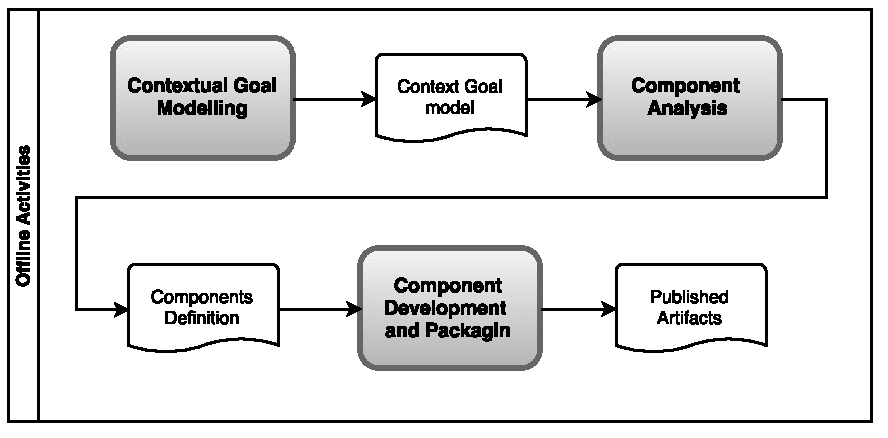
\includegraphics[width=\linewidth]{deployment_process_flow}
  \caption{Deployment Process Activities}
\label{fig:deployment_process_flow}
\end{figure}

\subsubsection{Goal Modeling}
This phase is coordinated by a requirement engineer with participation of a domain specialist, possibly the user.
A process such as TROPOS can be used. The output of this phase is a goal model.
Here, the goal model assumes a central role in the software development process. The goal model besides define the space of the solution, also works as common language. The goal model formalize the domain knowledge. It defines a common language between user and developers that will allow software deployment driven by user goals.


\subsubsection{Context Goal Modeling}
In this phase, the Goal model should be annotated with \emph{context conditions} related with the computing environment. That analysis is a context analysis and could benefit of the process described in~\cite{ali_goal-based_2010}. The requirements engineer should use knowledge about the computing resources that may be available at the computing environment.


\subsubsection{Component Analysis}
Software engineer should identify variability points.
Variability points in the contextual goal model are points where goals can be achieve with different strategies, each one having different context conditions.
Component interfaces are created following the guidelines described in Section~\ref{sec:rules}. The input and output of components are defined.

Also at this phase, it should be defined the sensors needed to evaluate facts about the computing environment.

\subsubsection{Component Development and Packaging}

Component development includes the cycle coding, build and test of software components.
The component package in the standard packaging schema is an artifact and should be put in a delivery system.
